%===================================== CHAP 2 =================================

\chapter{Neural Networks}
Object detection using complex machine learning techniques is possible due to the recent advances in image classification using convolutional neural networks and improvements in hardware. This chapter aims to give the reader an intuitive understanding of how a convolutional neural network works and how it classifies images, without going into too much depth. A more thorough explanation can be found in \citep{Krizhevsky2012}. The theory presented in this chapter is inspired by \citep{cnn_stanford}.

\section{Artificial Neural Networks}
A neural network is a group of neurons or nodes connected to each other. Each node can receive a signal from its input nodes, process it, and pass it on to its output nodes. In an Artificial Neural Network (ANN), the nodes are structured in layers, where there is one input layer, one output layer, and one or more hidden layers in between. When a node receives a signal it processes it using an \textit{activation function}, which defines the output of the node, given the input. The goal is to get the nodes to work together such that the network as a whole gives the correct output. A graphical representation can be seen in figure \ref{fig:NN}.

\begin{figure}
    \centering
    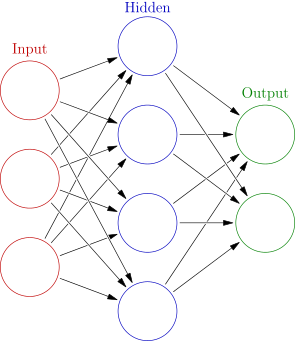
\includegraphics[scale=0.4]{fig/neural_network.png}
    \caption{Neural Network.}
    \label{fig:NN}
\end{figure}

\newpage

\subsection{Training of Neural Networks}
\label{sec:training}
The process of training neural networks is to tune the parameters of the activation function of each individual node such that the network as a whole gives the correct value as output. A simple example that would conform with figure \ref{fig:NN}, is input nodes where we have different features of a fish, e.g. its weight, color and age. The input nodes passes on the values of the fish features to the hidden layer, which processes the values using the activation function and passes on the value to the output nodes. The output nodes would be the fish type e.g. salmon and cod. Ideally, we want the value of the salmon output node to get the value 1 and the cod output node to get the value 0, if the inputted fish was in fact a salmon. Deviations from this result can be computed as a loss. We want to find the parameters for the activation functions in all the nodes that minimizes this loss. This is achieved by training the nodes on data where the class of the input object is known. If we have a data set of 1000 cods and 1000 salmons and their weight, color, and age we can use these as inputs, pass it through the network, and look at the loss. Then, by using gradient descent, we can change the parameters in all the activation functions in a way that makes the loss smaller. This is done using \textit{backpropagation}, which is an algorithm that calculates how the parameters in each activation function should be changed in order to reduce the loss. The idea is that doing this many times makes the network able to classify fish correctly, also on new data. 

%\vspace{3cm}

\section{Convolutional Neural Networks}

Convolutional neural networks are similar to ordinary neural networks, they too consist of nodes with activation functions structured into layers. What they do differently is that they assume that the input is an image, and use this assumption to do operations that are tailored for images, and improve both runtime and accuracy for image classification. 

\vspace{2mm}

If we want to process an image through an artificial neural network, we would transform the image into a vector, where each row of the image now is in one large row. That would mean that color images, which has three channels (RGB), of size 256 x 256 would have 256 x 256 x 3 = 196,608 neurons in the first hidden layer. Convolutional neural networks reduces the number of neurons by using \textit{convolutional layers} and \textit{pooling layers}.

\subsection{Convolutional Layers}
\label{sec:conv}
 A convolutional layer consists of a set of filters. When a convolutional layer receives an image input, it slides, or convolves, filters over all the pixels in the input image and output the dot product of the filter and the image at the filters position. This will create an activation map, where we can see the response of the filter at different positions. During training the different filters will change in order to detect different things in the input image. Imagine we want to classify images of handwritten ones and zeros. Some filters may aim to detect the rounded shape of the zeros, and will therefore output a large number if it detects a rounded shape. Figure \ref{fig:filter_cnn} illustrates this. The figure shows two example filters, filter 1 detects vertical lines, while filter 2 detects upper left regions of circles. 

\begin{figure}[h!]
    \centering
    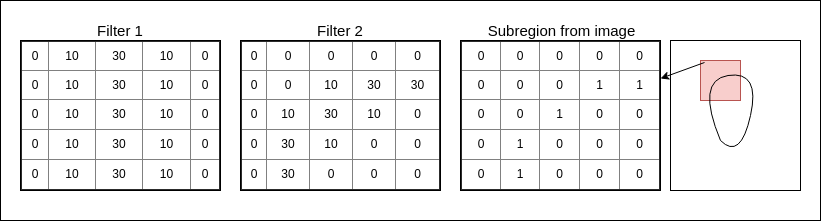
\includegraphics[scale=0.40]{fig/Filter_cnn.png}
    \caption{Filter and subregion of an image of a handwritten zero, in the \textit{Subregion from image} the ones represent pixels that are black, the zeros represent pixels that are white.}
    \label{fig:filter_cnn}.
\end{figure}

\newpage

The dot product, or the activation of the two filters at this position in the image is $30 \cdot 1 + 10 \cdot 1 + 10 \cdot 1 + 10 \cdot 1 = 60$ for filter 1, and $30 \cdot 1 + 30 \cdot 1 + 30 \cdot 1 + 30 \cdot 1 + 30 \cdot 1 = 150$ for filter 2. This means that the activation map for filter 2 is much higher than for filter 1 at this position. For a different subregion the result would be different. When we have several different filters they will activate at different positions and thus have different activation maps. Combining the the different activation maps for the different filters tells us something about the image as a whole. During training of a convolutional neural network, the network is trained to draw conclusions of what is in the image based on which filters activate at which positions. 

\vspace{2mm}


\subsection{Pooling Layers}
The pooling layers are downsampling layers. They work by sliding boxes of e.g. 2x2 over the pixels of the image, and process the values to output a single value for those 4 pixels. There are different ways to process the pixels, where \textit{max pooling} is a commonly used method. An example of how to downsample an image by a factor of two using max pooling is shown in figure \ref{fig:max_pool}.

\begin{figure}[h!]
    \centering
    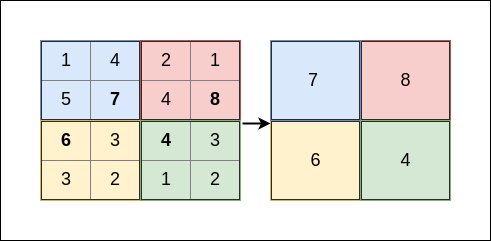
\includegraphics[scale=0.42]{fig/pooling.png}
    \caption{Max pooling.}
    \label{fig:max_pool}
\end{figure}

Max pooling transforms the pixels inside the sliding box into one pixel with the same value as the highest pixel value in the original box. By downsampling the image the number of parameters is reduced, which in turn reduces the computational cost of the algorithm. The pooling layers usually follow a convolutional layer, and can therefore help the next convolutional layer pick up features the previous layer could not. Pooling layers can also help preventing overfitting, which is when a classification algorithm performs well on training data, but badly on test data.

\section{Transfer Learning}
Transfer learning is a machine learning method where a network trained on one task is repurposed on a second similar task, and is a technique used extensively in this project. A problem in deep learning is \textit{data dependence}, meaning that deep learning processes depends on a massive training dataset to be able to understand the patterns in the data \citep{TransferLearning2}. This is especially a problem in deep learning compared to traditional machine learning methods, since deep learning methods have to learn features from the dataset, while in traditional machine learning methods the user has to design the features. 

\vspace{3mm}

To counter the \textit{data dependence} of a neural network one needs a large well-annotated dataset, which may be both costly and time consuming to acquire \citep{TransferLearning}. Transfer learning provides a way of utilizing training data that does not conform with the test data. 


Meaning that e.g. a classifier trained to detect dogs can be retrained to detect ducks, saving training time and training data requirements compared to training a duck classifier from scratch. 



\begin{figure}[h!]
    \centering
    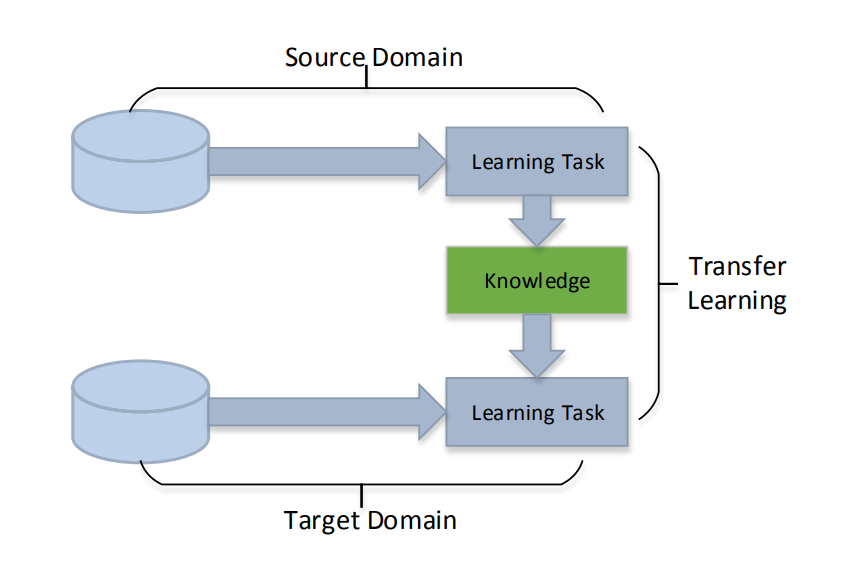
\includegraphics[scale=0.4]{fig/transfer_learning.png}
    \caption{Transfer learning, figure from \citep{TransferLearning2}}
    \label{fig:transfer_learning}
\end{figure}

Figure \ref{fig:transfer_learning} shows how data from the source domain is used to train a classifier, then using this knowledge in combination with data from the target domain to train a new classifier. 

\vspace{3mm}

\citep{TransferLearning2} categorized network-based deep transfer learning into the following four methods.

\begin{outline}
    \1 Instances-based
       \2 Supplement the training data in the target domain with relevant instances from the source domain by assigning fitting weights to the selected values.
    \1 Mapping-based
       \2 Maps instances from the source domain and the target domain to a new data space. The reasoning for this is: "Although there are differences between the two origin domains, they can be more similar in an elaborate new data space." \citep{TransferLearning2}
    \1 Network-based
       \2 Reuses parts of the network that is pre-trained on the source domain. The target domain retrains the last part of the network on new data while keeping the weights in the other layers. The idea is that the first layers in neural network finds more general features, while the last layers narrows down to the features specific for the class of interest. A classifier trained on images of boats and a classifier trained on cars may detect similar features in the first layers of the network. This is the transfer learning method used in this project.
    \1 Adversial-based
       \2 Finds transferable features that are suitable in both target domain and source domain
\end{outline}



\cleardoublepage